\chapter{Bearbeitung der Aufgaben}
\section{Geschichteter Plattenkondensator}

Um numerisch die Kapazität eines Plattenkondensators mit quer geschichteten Dielektrika, die eine linear steigende relative Permittivität aufweisen, zu bestimmen, kann man den linearen Verlauf über mehrere Schichten mit jeweils konstanter Permittivität approximieren. Wie bei numerischen Verfahren üblich wird die Approximation besser, je dünner die einzelnen Schichten gewählt werden.\\
\begin{figure}[h!]
	\centering
	\begin{subfigure}[h]{0.3\textwidth}
		\centering
		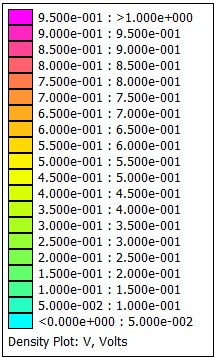
\includegraphics[width=\textwidth]{data/KondensatorN9_Legende}
		\caption{Skala}
		\label{fig:Skala1}
	\end{subfigure}
	\begin{subfigure}[h]{0.51\textwidth}
		\centering
		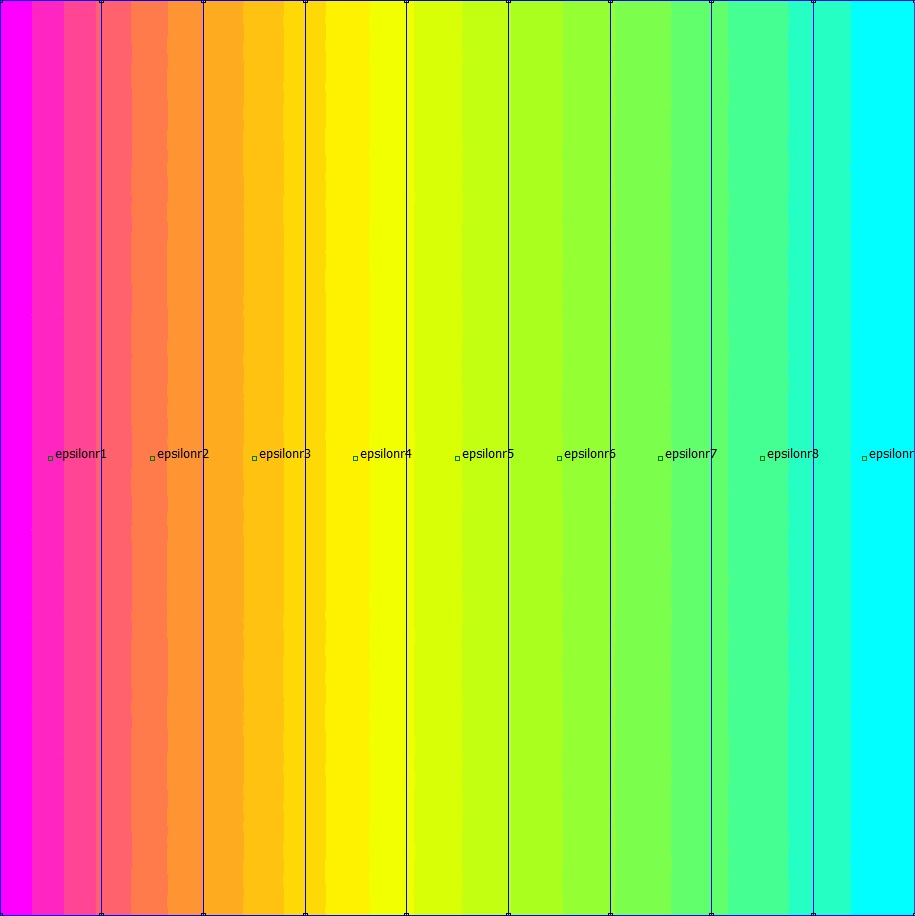
\includegraphics[width=\textwidth]{data/KondensatorN9}
		\caption{Potentialverlauf im Plattenkondensator mit 9 Schichten}
		\label{fig:N9}
	\end{subfigure}
	\caption{Potentialverlauf im Plattenkondensator mit 9 Schichten}
\end{figure} \\
Die Funktion \texttt{femmcapacity.m} bekommt als Parameter den Abstand $h$ zwischen den beiden Platten des Kondensators, die Kantenlänge $a$ der quadratischen Platten, $\varepsilon_{\mathrm{r,1}}$, $\varepsilon_{\mathrm{r,2}}$ und die Anzahl $N$ an Schichten übergeben. Mit Hilfe dieser Parameter wird daraus ein Plot für den Potentialverlauf im Kondensator erzeugt und die Kapazität der Anordnung berechnet. Die relative Permittivität variiert hierbei linear zwischen $\varepsilon_{\mathrm{r,1}} $ am linken Rand und $\varepsilon_{\mathrm{r,2}}$ am rechten Rand. Die zugehörigen Werte der relativen Permittivitäten der einzelnen Schichten $N_i$ lassen sich mit $$ \varepsilon_{\mathrm{r,i}} = \varepsilon_{\mathrm{r,1}} + \frac{i (\varepsilon_{\mathrm{r,2}}-\varepsilon_{\mathrm{r,1}})}{N-1}$$ berechnen. Im Folgenden wird der Abstand zwischen den Platten und die Kantenlänge mit \SI{30}{\centi\meter} angenommen. Wählt man 9 Schichten, $\varepsilon_{\mathrm{r,1}} = 1$ und $\varepsilon_{\mathrm{r,2}} = 2$  erhält man den in Abbildung \ref{fig:N9} zu sehenden Potentialverlauf und eine Kapazität $ C_1 = \SI{3,793}{\pico\farad}$.\\ \\
Wiederholt man die Simulation für $N = 1,2,3,...,20$ Schichten und lässt sich in einem Konvergenz-Plot (Abbildung \ref{fig:semilogy}) die Kapazität in Abhängigkeit der Schichtanzahl anzeigen, wird deutlich, dass schon nach $N=3$ Schichten die Kapazität annähernd exakt bestimmt wird und weitere Verfeinerungen nur noch marginale Verbesserungen der Approximation erzielen. \\ \\

\begin{figure}[tpbh]
	\centering
	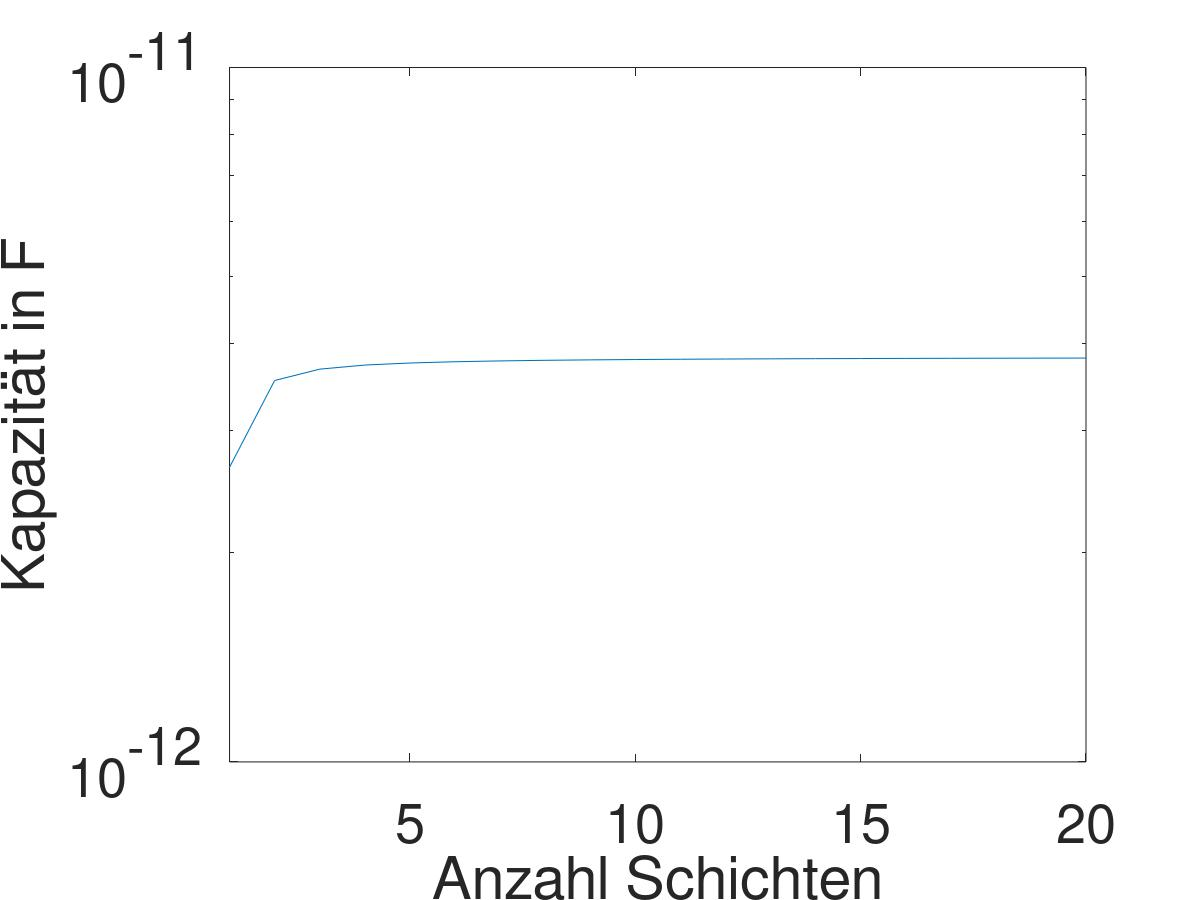
\includegraphics[width=.8\textwidth]{data/Kapazitaet}
	\caption{Änderung der Kapazität mit steigender Anzahl an Schichten im Plattenkondensator}
	\label{fig:semilogy}
\end{figure}


Die Option \texttt{'Vector Plot'} in FEMM ist nützlich, um den Verlauf des elektrischen Feldes besser darzustellen. Die Richtung der Pfeile zeigt an in welche Richtung das Feld an dieser Stelle zeigt und die Länge der Pfeile deutet die Stärke an dieser Stelle an.
\newpage
In Abbildung \ref{fig:N1_EFeld} sieht man den Plot für den homogenen Plattenkondensator und in Abbildung \ref{fig:N9_EFeld} für den geschichteten Fall. Vergleicht man beide Abbildungen fällt auf, dass das elektrische Feld im homogenen Plattenkondensator homogen verteilt ist. Beim geschichteten Plattenkondensator hingegen ist das elektrische Feld deutlich stärker auf der Seite mit der geringeren relativen Permittivität und nimmt immer weiter ab, je höher die relative Permittivität ist.

\begin{figure}[h]
	\begin{subfigure}[c]{0.2\textwidth}
		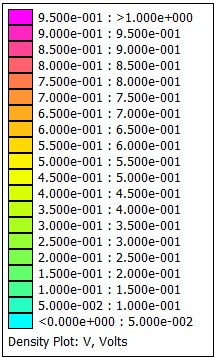
\includegraphics[width=\textwidth]{data/KondensatorN9_Legende}
		\caption{Skala}
		\label{fig:Skala2}
	\end{subfigure}
	\begin{subfigure}[c]{0.35\textwidth}
		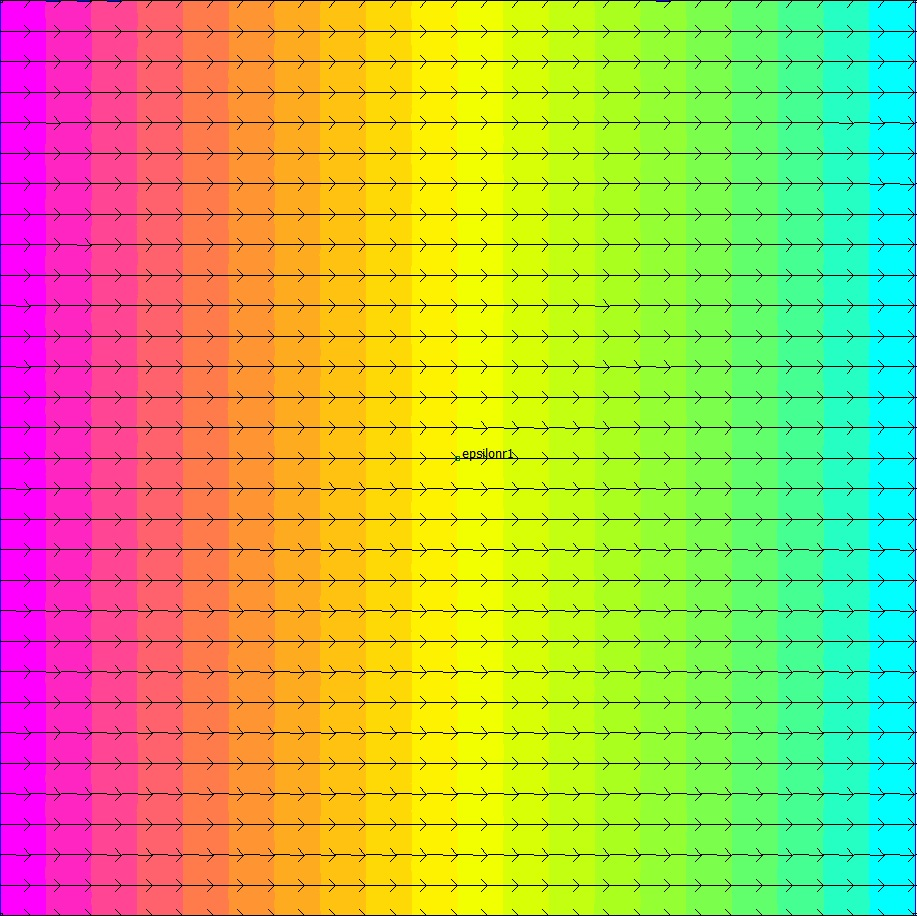
\includegraphics[width=\textwidth]{data/KondensatorN1_EFeld}
		\caption{Potentialverlauf und elektrische Feldstärke im homogenen Plattenkondensator}
		\label{fig:N1_EFeld}
	\end{subfigure}
	\begin{subfigure}[c]{0.35\textwidth}
		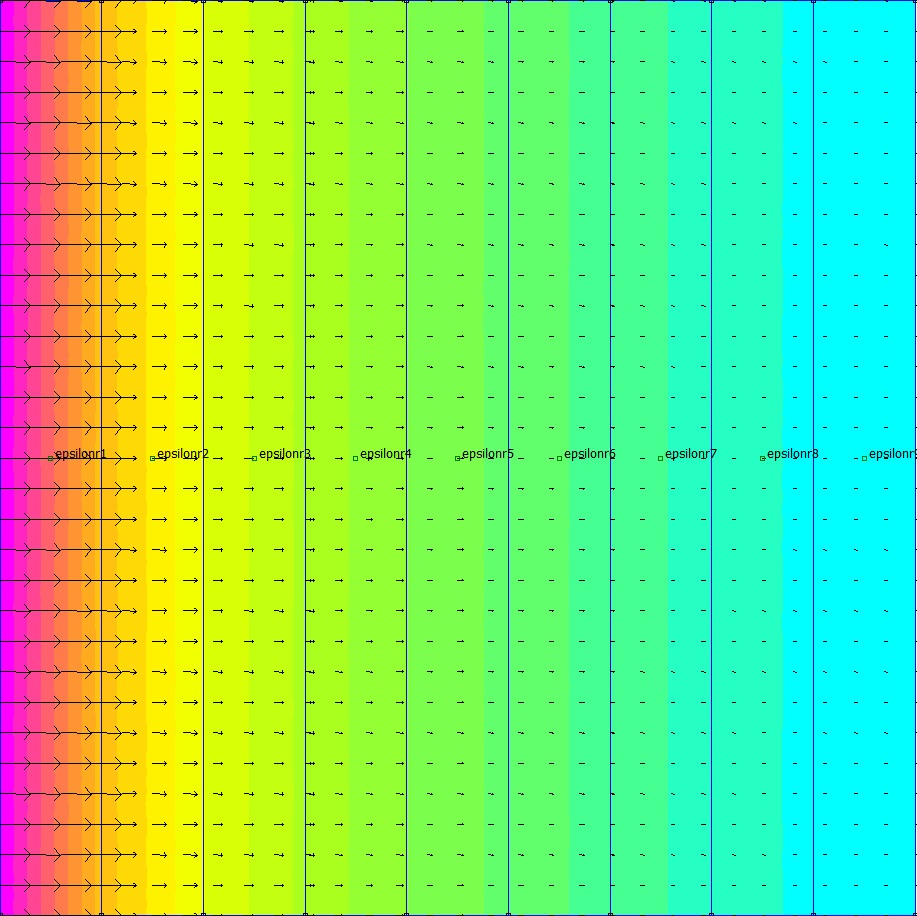
\includegraphics[width=\textwidth]{data/KondensatorN9_EFeld}
		\caption{Potentialverlauf und elektrische Feldstärke im Plattenkondensator mit 9 Schichten}
		\label{fig:N9_EFeld}
\end{subfigure}
	\caption{Potentialverlauf und elektrische Feldstärke im homogenen und im geschichteten Plattenkondensator}
\end{figure}

Bestimmt man die Kapazität für $\varepsilon_{\mathrm{r,1}} = 1$ und $\varepsilon_{\mathrm{r,2}} = 10$ und $N = 9$ und vergleicht diese mit der vorher bestimmten Kapazität $C_1$ stellt man fest, dass durch eine höhere relative Permittivität auch die Kapazität von $\SI{3,793}{\pico\farad}$ auf $\SI{8,916}{\pico\farad}$ steigt.

